\documentclass{article}
\usepackage{xcolor}
\usepackage{graphicx}
\usepackage{float}
\usepackage{tikz}
\usepackage{parskip}
\usepackage{amsmath}
\usepackage{amsthm}
\usepackage{amssymb}
\usepackage{mathtools}
\usepackage{fancyhdr}
\usepackage[%paperheight = 59.4cm,
            %paperwidth = 42cm,
            %includehead,
            nomarginpar,
            textwidth=15cm,
            headheight=10mm]{geometry}


\begin{document}
 
\pagestyle{fancy}
%\fancyhead{}\fancyfoot{}

\fancyhf[OHC]{Christopher Munoz WRH2 Optimization}
\textbf{Problem 2.4:} \\
We are given the following expression and are tasked with graphing the feasible set and determining any local or global minimizers:
\begin{align*}
    \text{minimize} &\null \quad f(x) = x_1 \\
    \text{subject to} &\null \quad (x_1 - 1)^2 + x_2^2 = 1 \\ 
    &\null \quad (x_1+1)^2 + x_2^2 = 1
\end{align*}
Below is the graph of the feasible set:

\begin{figure}[H]
    \centering
    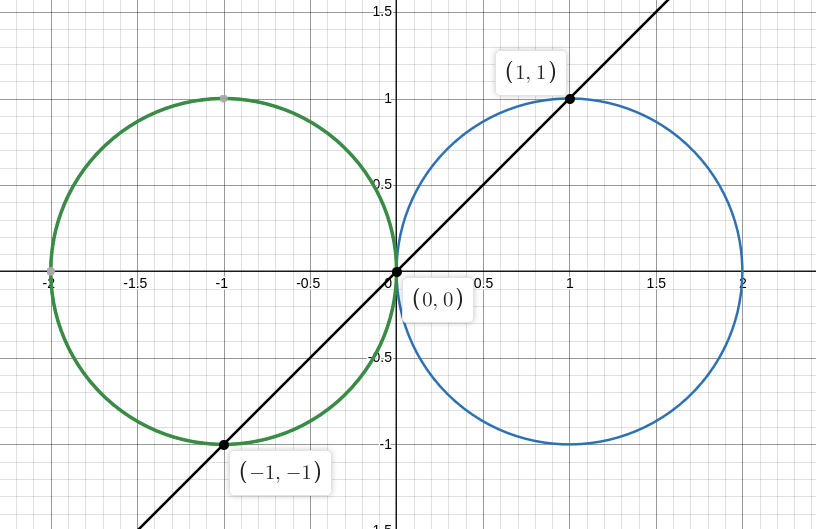
\includegraphics[scale = 0.40]{desmos1.png}
\end{figure}
Because our objective function is linear, the local minimizer and the global minimizer are the same value. We determine that (-1, -1) is both our global and local minimizer.
\break
\break
\textbf{Problem 2.5:} In this exercise we are tasked with providing an example function that nas no global minimizer and no global maximizer. If we take any linear function without constraints we will have no global minimizer or maximizer. The function $f(x) = x_1$ for example.
\break \break
\textbf{Problem 2.7:} Theorem: Given $f(x)$ for $x \in S$ and $S$ is the set of all integers, Every point in $S$ is a local minimizer in $f$.
\newline
Proof: First note that since $x \in S$, then $x-1$ and $x+1$ must also be in S.  Suppose x is a local minimizer, replacing x with the values of $x-1$ or $x+1$ should yield us values greater than $f(x)$. Then we know that $f(x) \leq f(x+1)$ and $f(x) \leq f(x-1)$ by definition of local minimizer. 
\break \break
\textbf{Problem 3.1:} Theorem: The intersection of a finite number of convex sets is also a convex set.
\newline Proof: Suppose $S$ is the intersection of a finite number of convex sets and $S \subseteq \mathbb{R}^n$. We will show that $S$ is also convex. Let $G_1, G_2, ... , G_n$ be convex sets where $G_1, G_2, ... , G_n = S$, let $x, y \in S$ and $\alpha \in [0,1]$. We want to show that $\alpha x + (1-\alpha)y \in S$, Since $x,y \in S$, then $x,y \in G_i$ for all $i$ in $ \{1, 2, ..., n\} $. This would mean that $\alpha x + (1 - x)y$ is in $G_i$ for all $i$ in $\{1,2,...,n\}$. Thus $\alpha x + (1 - x)y \in S$, therefore proving that the interesection of a finite number of convex sets is itself convex.
\break
\break
\textbf{Problem 3.3:} Theorem: Given the feasible region S defined by a set of linear constraints
\begin{align*}
    S = \{ x : Ax \leq b \}
\end{align*}
$S$ is convex.
\newline Proof: For a $S$ to be convex then $S$ must satisfy $x,y \in S$ and $\alpha x + (1 - \alpha) \in S$ where $\alpha \in [0,1]$, also $S$ is a subset of $\mathbb{R}^n$.  Suppose $Ax \leq b$ and $Ay \leq b$, we consider the following:
\begin{align*}
    A(\alpha x + (1 - \alpha)y) & = A\alpha x + (1 - \alpha)Ay \\
    & \leq \alpha b + (1 - \alpha)b \\
    & \leq \alpha b + b - \alpha b \\
    & \leq  
\end{align*}
This shows that our region S defined by a set of set of linear constraints $S = \{ x : Ax \leq b \}$ is convex.
\break
\break
\textbf{Problem 3.7:}
\end{document}
